\documentclass[10pt]{beamer}

\usepackage{settings}


\title{From Latent to Deep Latent Variable Models}
\subtitle{A Study On Causal Effect Inference with CEVAE}
\date{June 17, 2025}
\author[longname]{Valeria De Stasio, Christian Faccio, Giovanni Lucarelli}
\titlegraphic{\hfill
\includegraphics[height=1.3cm]{images/logo100_orizzontale.pdf}}

% add graphics path
\graphicspath{{../assets},{./images}}

\begin{document}

\maketitle

% magari un frame iniziale in cui introduciamo il concetto di causalità?
\begin{frame}{Objective: estimating causal effects}
    Estimate how a medical treatment $T$ affects the health $Y$ of a \textit{random} patient.
  \begin{figure}
    \centering
    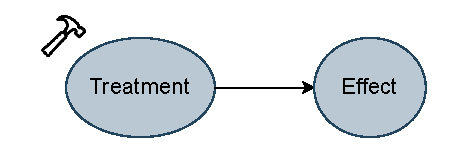
\includegraphics[width=0.7\textwidth]{images/no_confounders.pdf}
  \end{figure}

  \begin{equation*}
    P(Y=y|\text{do}(T=t))=P(Y=y|T=t)
  \end{equation*}
  \begin{equation*}
    \text{ITE} = \mathbb{E}[(Y|\text{do}(T=1)]-\mathbb{E}[(Y|\text{do}(T=0)]
  \end{equation*}
  
  This is usually the case in a \textbf{randomized controlled trial} (RCT), where the treatment is randomly assigned to the patients.

\end{frame}


% How to intervene on already observed data?
\begin{frame}{Confounder}
  In a observational study:
  \begin{itemize}
    \item \textbf{no} control over the treatment $T$ assignment\\
    $\rightarrow$ there may be a confounder $X$ (e.g. Income) that influences both variables
  \end{itemize}
  \begin{columns}
    \begin{column}{0.5\textwidth}
      \begin{equation*}
        P(Y|\text{do}(t))\ne P(Y|t)
      \end{equation*}
      \begin{equation*}
        P(Y|\text{do}(t),x) =P(Y|t,x)
      \end{equation*}
    \end{column}
    \begin{column}{0.5\textwidth}
      \begin{figure}
        \centering
        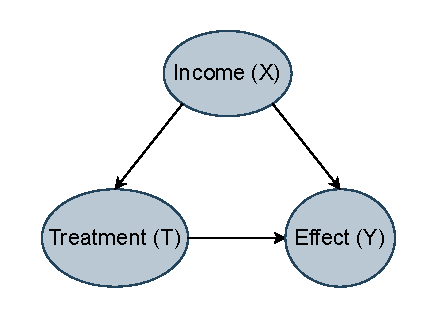
\includegraphics[width=\textwidth]{images/unconfoundness.pdf}
      \end{figure}
    \end{column}
  \end{columns}

  \centering{If the confounder is observed even a linear rergession can do the job!}
\end{frame}

\begin{frame}{Latent confounder}
But what if the confounder $Z$ (e.g. Wealth) is \textbf{not} observed and the observed $X$ is only a proxy of it?
    \begin{center}
  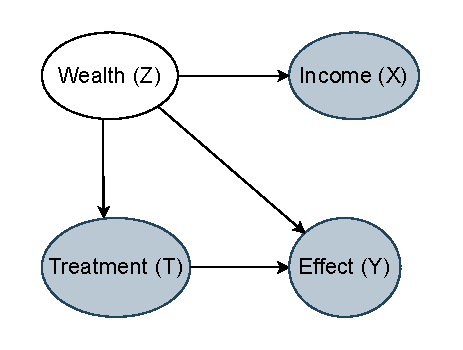
\includegraphics[width=0.5\textwidth]{images/latent_confounder.pdf}
\end{center}
  
\textbf{Idea:} estimate the latent variable and condition on it
% \begin{itemize}
%     \item Latent Variable Model
%     \item Deep Latent Variable Model
% \end{itemize} 

 \end{frame}


 \begin{frame}{Vanilla Latent Variable Model}
     \begin{itemize}
         \item \textbf{Generative model:}
         \begin{columns}
              \begin{column}{0.75\textwidth}
                  \begin{equation*}
                    Z \sim \mathcal{N}(0,\,1)
                  \end{equation*}
                  \begin{equation*}
                    X_j \sim \mathcal{N}(a\,z + b,\; \text{diag}(\sigma_X^2))
                  \end{equation*}
                  \begin{equation*}
                    T \sim \mathrm{Be}(\sigma(c\,z))
                  \end{equation*}
                  \begin{equation*}
                    Y \sim \mathcal{N}(e\,t + f\,z,\,\sigma_Y^2)
                  \end{equation*}
              \end{column}
              \begin{column}{0.5\textwidth}
                  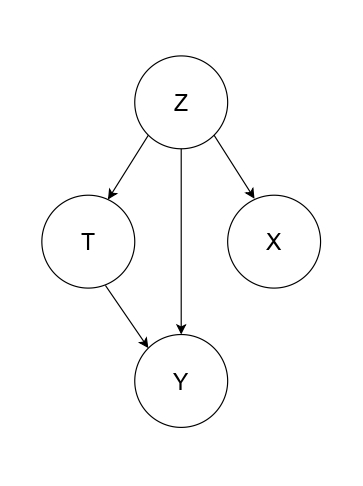
\includegraphics[width=0.5\textwidth]{images/model.jpg}
              \end{column}
         \end{columns}

         \item \textbf{Guide:} mean-field assumption over the observations
        %  \item For a new data point $x$:
        %  \begin{itemize}
        %      \item infer: $z_0 =\mathbb{E}[Z|x,T=0]$, $z_1=\mathbb{E}[Z|x,T=1]$
        %      \item compute $\text{ITE} = \mathbb{E}[Y|T=1,z_1]-\mathbb{E}[Y|T=0,z_0]$
        %  \end{itemize}
          \item \alert{\textbf{Problem:}} we need to train a new model at test time!
     \end{itemize}
 \end{frame}


 \begin{frame}{From Latent to Deep Latent}
  \begin{columns}
    \begin{column}{0.5\textwidth}
      \textbf{Latent Variable Model} (LVM):
      \begin{itemize}
        \item Linear functions
        \item SVI + mini-SVI for new x
        \item Small number of parameters
        \item High interpretability
      \end{itemize}
    \end{column}
    \begin{column}{0.5\textwidth}
      \textbf{Deep Latent Variable Model} (CEVAE):
      \begin{itemize}
        \item MLP functions
        \item SVI + Amortized inference
        \item Large number of parameters
        \item High flexibility
      \end{itemize}
    \end{column}
  \end{columns}
  \vspace{1cm}
  \centering{\textbf{CEVAE} = LVM + MLPs + Amortized Inference\\ 
  same causal idea, more flexibility and speed at test time.}
\end{frame}


  \begin{frame}{Deep Latent Variable Model: CEVAE}
    %  \begin{itemize}
    %      \item Assume parametric relationships between variables through \alert{Neural Networks}
         
    %      \item \textbf{CEVAE} = VAE + causal semantics for latent \(Z\)  
    %         \[
    %           (X,\;T,\;Y)\longrightarrow\;Z \;\longrightarrow\; (X,\;T,\;Y)
    %         \]
    %   \item Counterfactuals in one forward pass  \(\Rightarrow\) \textbf{amortized inference, no test-time training}
    %  \end{itemize}
    \begin{center}
  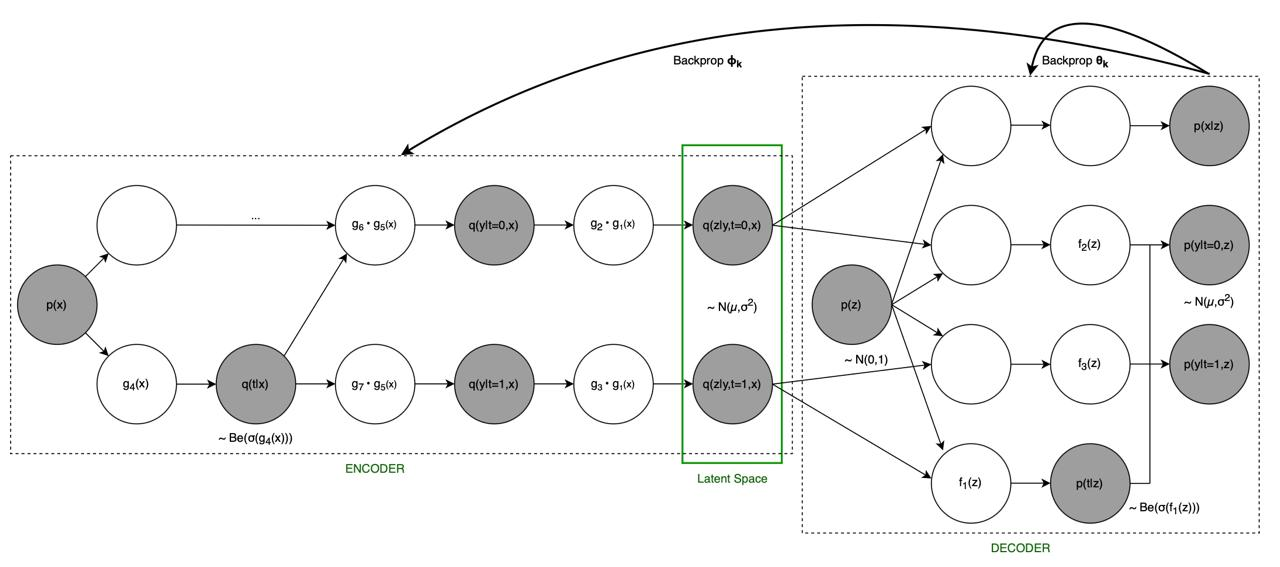
\includegraphics[width=0.9\textwidth]{images/cevae_architecture.jpeg}
\end{center}

 \end{frame}




\begin{frame}{Synthetic linear dataset}
    \begin{minipage}{0.48\textwidth}
      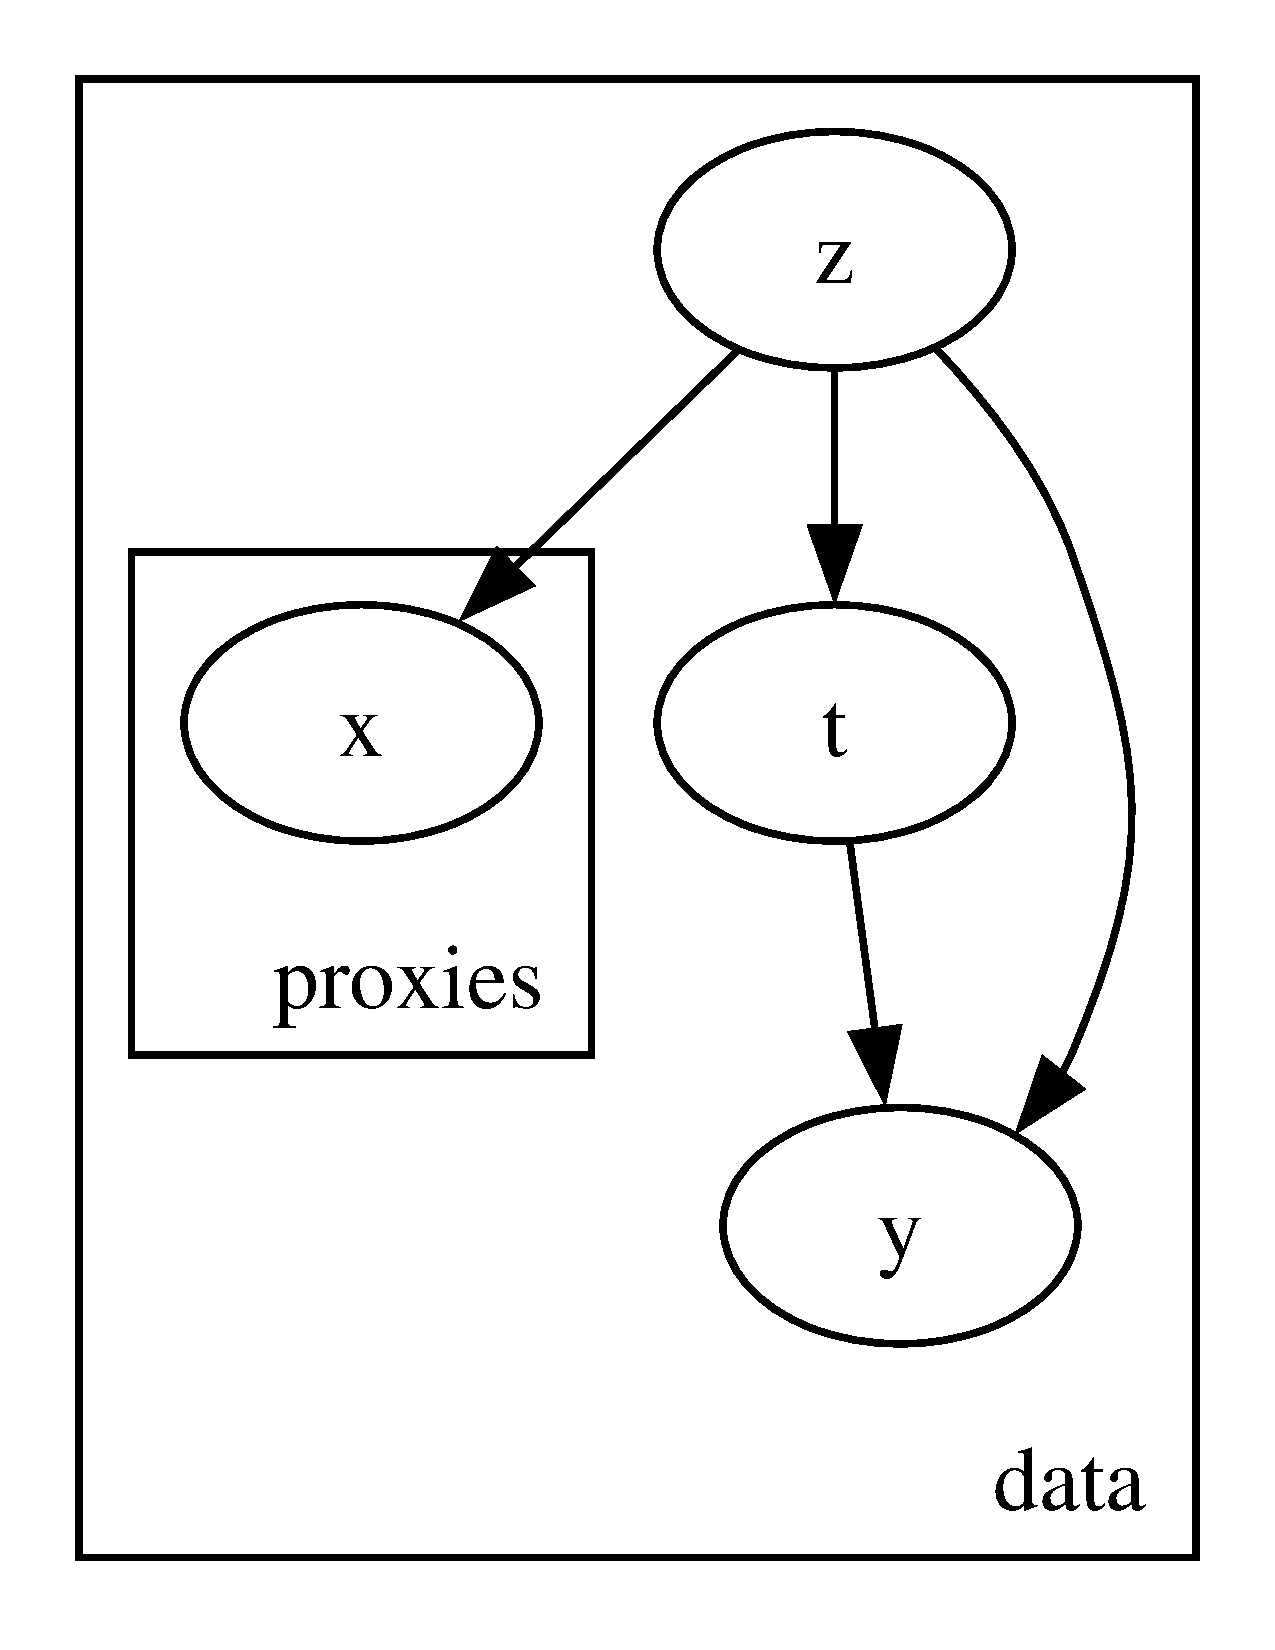
\includegraphics[width=0.9\textwidth]{images/pyro_model.pdf}
    \end{minipage}
    \begin{minipage}{0.48\textwidth}
        \begin{equation*}
        Z \sim \mathcal{N}(0,1)
        \end{equation*}
        \begin{equation*}
             a_j \sim \mathcal{U}(-10,10)
        \end{equation*}
        \begin{equation*}
        X_j \sim \mathcal{N}(a_j z,\sigma_X^2)\,    
        \end{equation*}
        \begin{equation*}
        T | Z \sim \mathrm{Be}(\sigma(\beta z))    
        \end{equation*}
        \small{\begin{equation*}
        Y|T,Z \sim \mathcal{N}(z + t, \sigma_Y^2)            
        \end{equation*}}
      \end{minipage}
      \centering
      {\textbf{Remark:} ITE is constant for all  $x$!}
\end{frame}

\begin{frame}{Synthetic non linear dataset}
    \begin{minipage}{0.48\textwidth}
    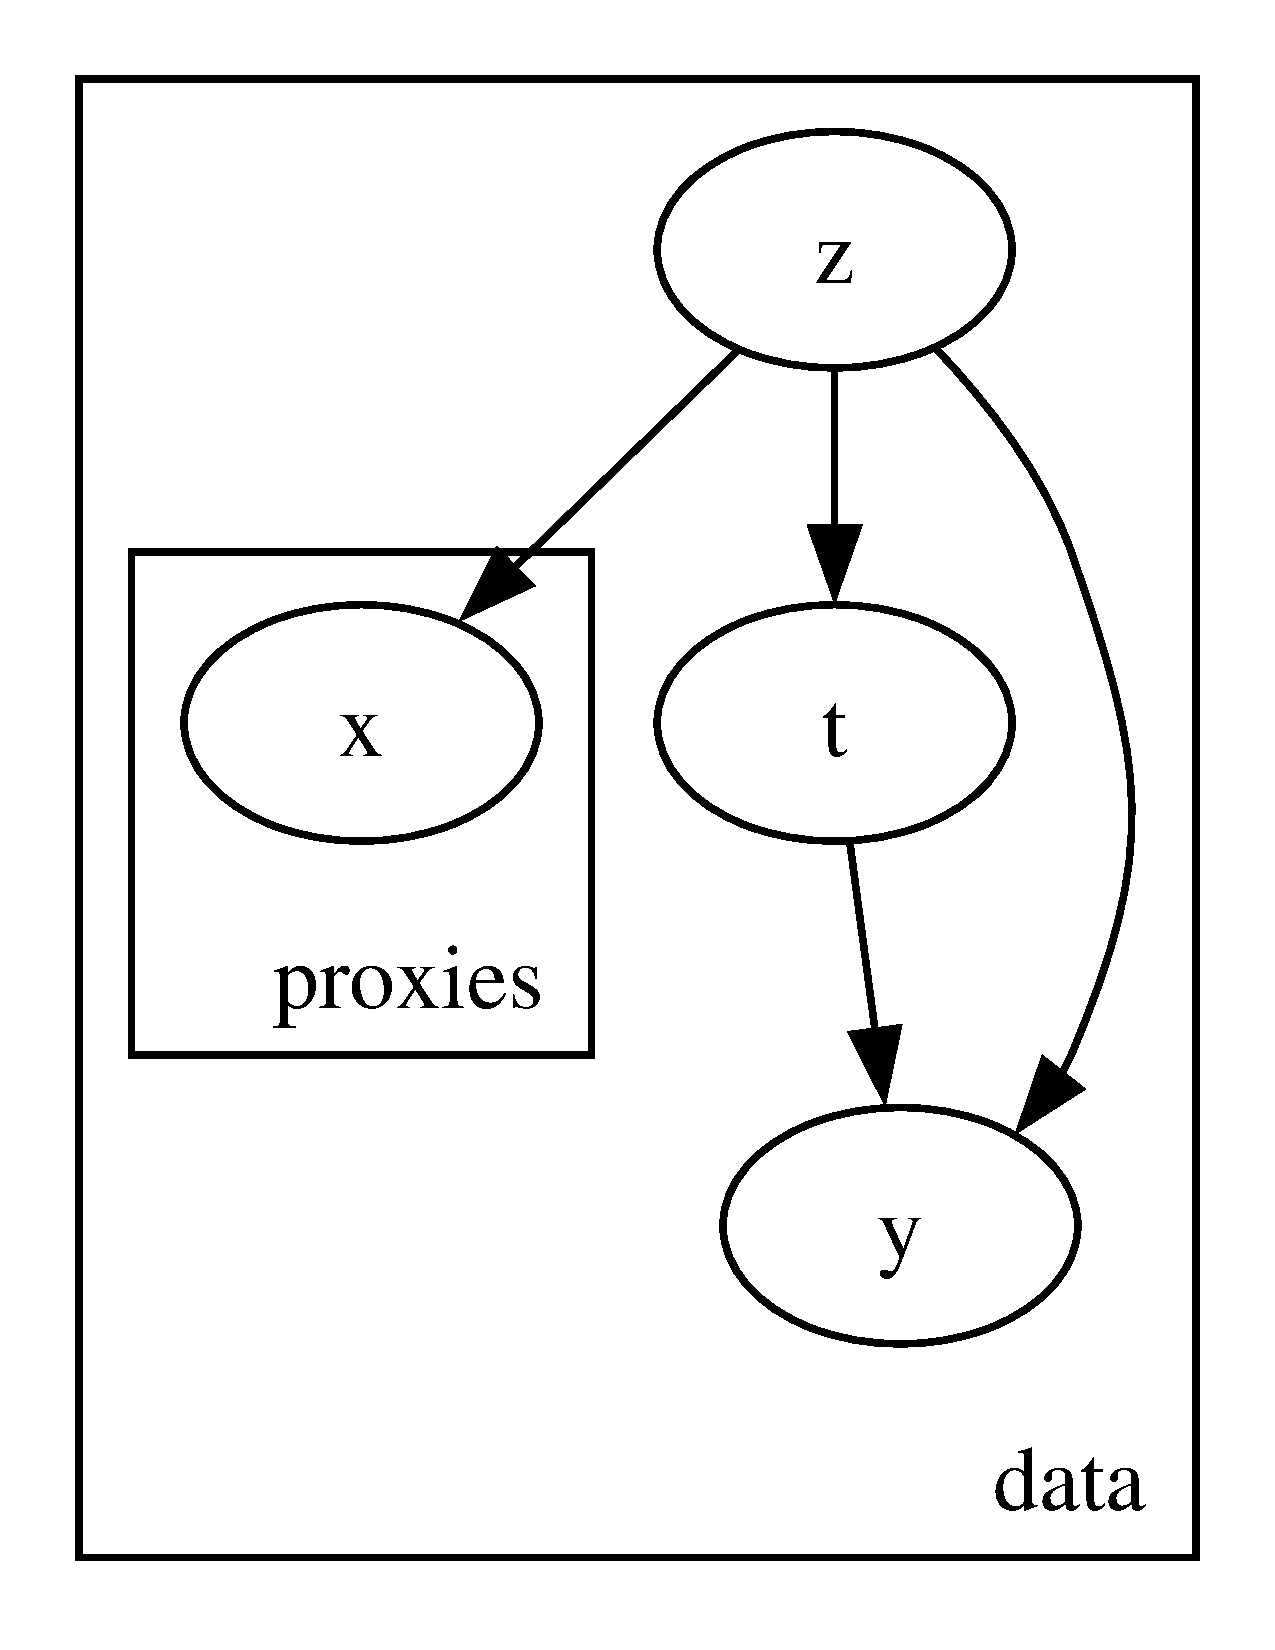
\includegraphics[width=0.9\textwidth]{images/pyro_model.pdf}
    \end{minipage}
    \begin{minipage}{0.48\textwidth}
    
        \begin{equation*}
        Z \sim \mathcal{N}(0,1)
        \end{equation*}
        \begin{equation*}
            a \sim \mathcal{U}(-10,10)^d
        \end{equation*}
        \begin{equation*}
        X_1,...,X_d \sim \mathcal{N}(a\tanh(z),\sigma_X^2\mathbb{I} )     
        \end{equation*}
        \begin{equation*}
        T | Z \sim \mathrm{Be}(\sigma(\beta z))    
        \end{equation*}
        \begin{equation*}
        Y|T,Z \sim \mathcal{N}\left(\text{NonLin}(z,t),\sigma_Y^2\right)           
        \end{equation*}
        \begin{equation*}
        \text{NonLin}(z,t) = \sin(z)+\frac12z+t\left(1+\frac12z\right)      
        \end{equation*}
    \end{minipage}
    \centering
    {\textbf{Remark:} ITE depends on interaction between $t$ and $z$!}
\end{frame}

\begin{frame}{Results (1/2): Linear Dataset}
    \begin{figure}[H]
      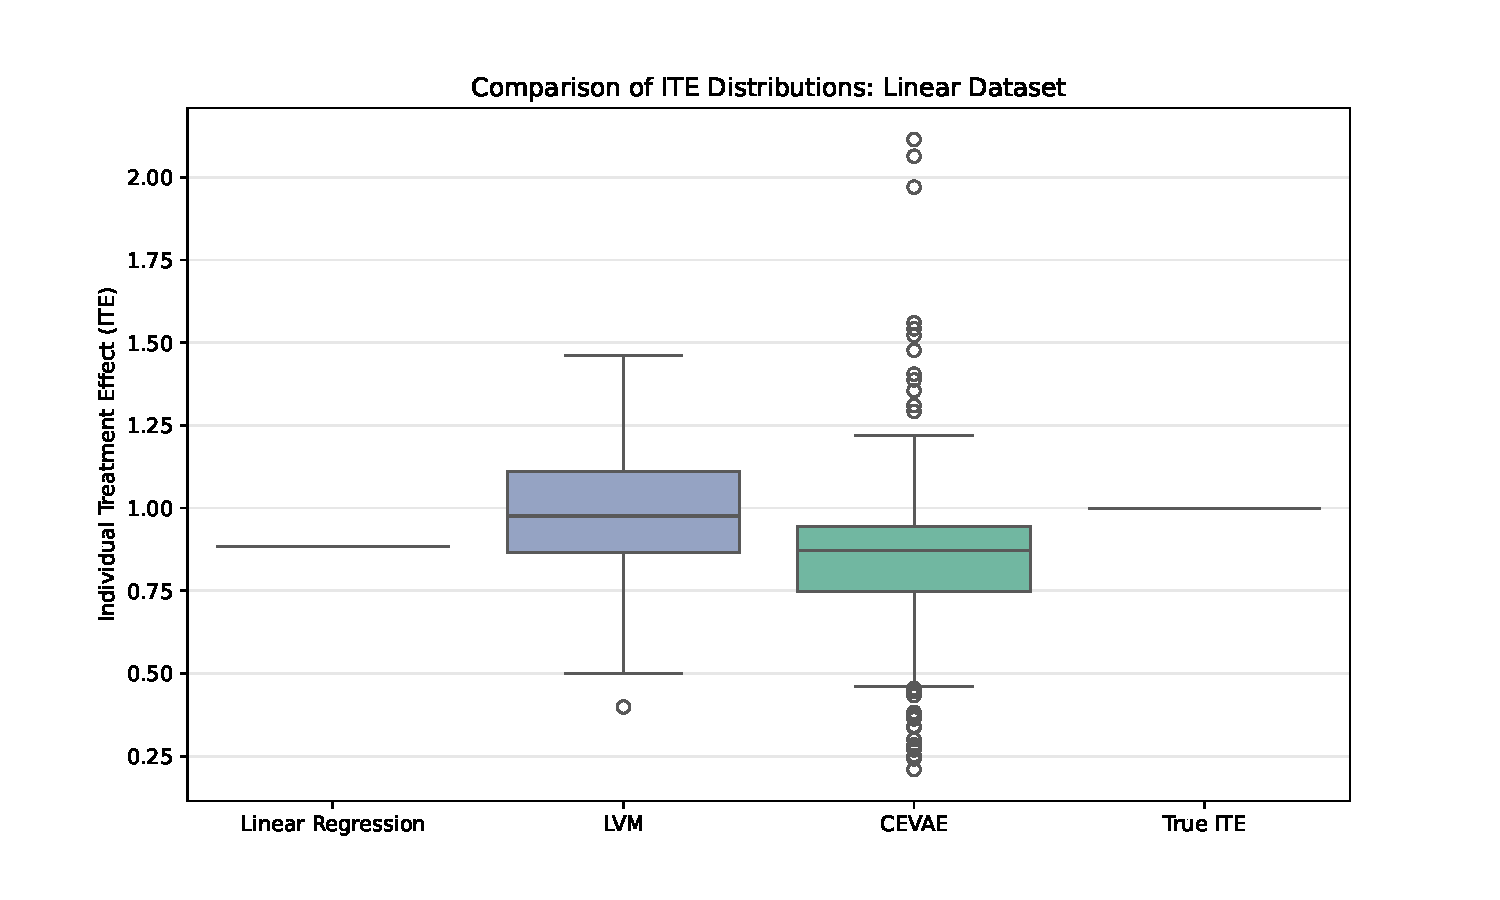
\includegraphics[width=\textwidth]{images/boxplot_linear.pdf}
    \end{figure}
\end{frame}

\begin{frame}{Results (2/2): Non Linear Dataset}
    \begin{figure}[H]
      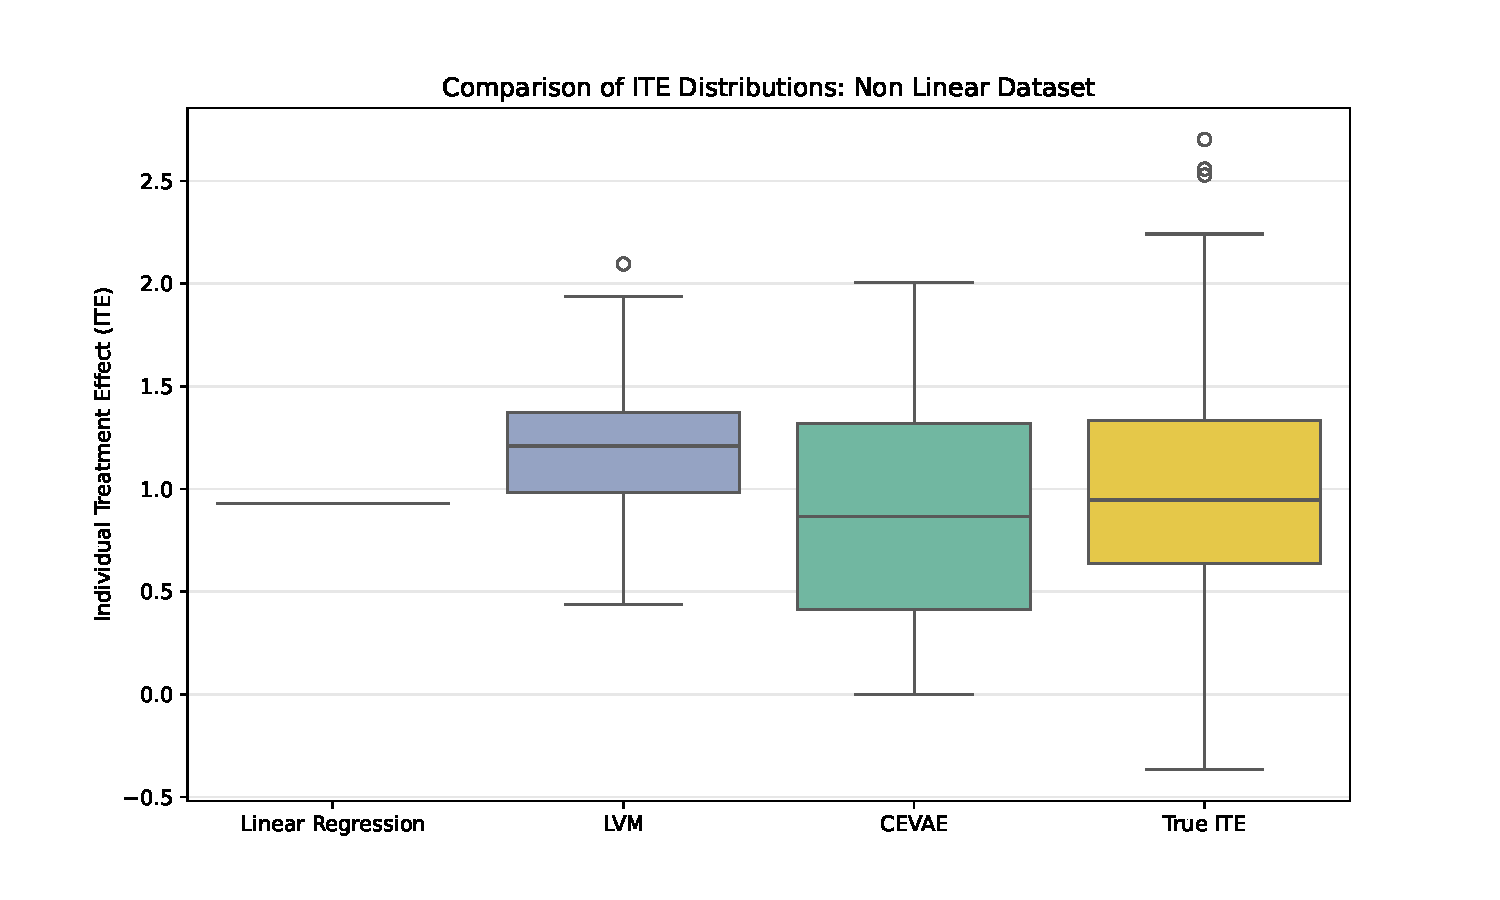
\includegraphics[width=\textwidth]{images/boxplot_non_linear.pdf}
    \end{figure}
\end{frame}

\begin{frame}{Internal Representation: Linear Dataset}
  \begin{figure}[H]
    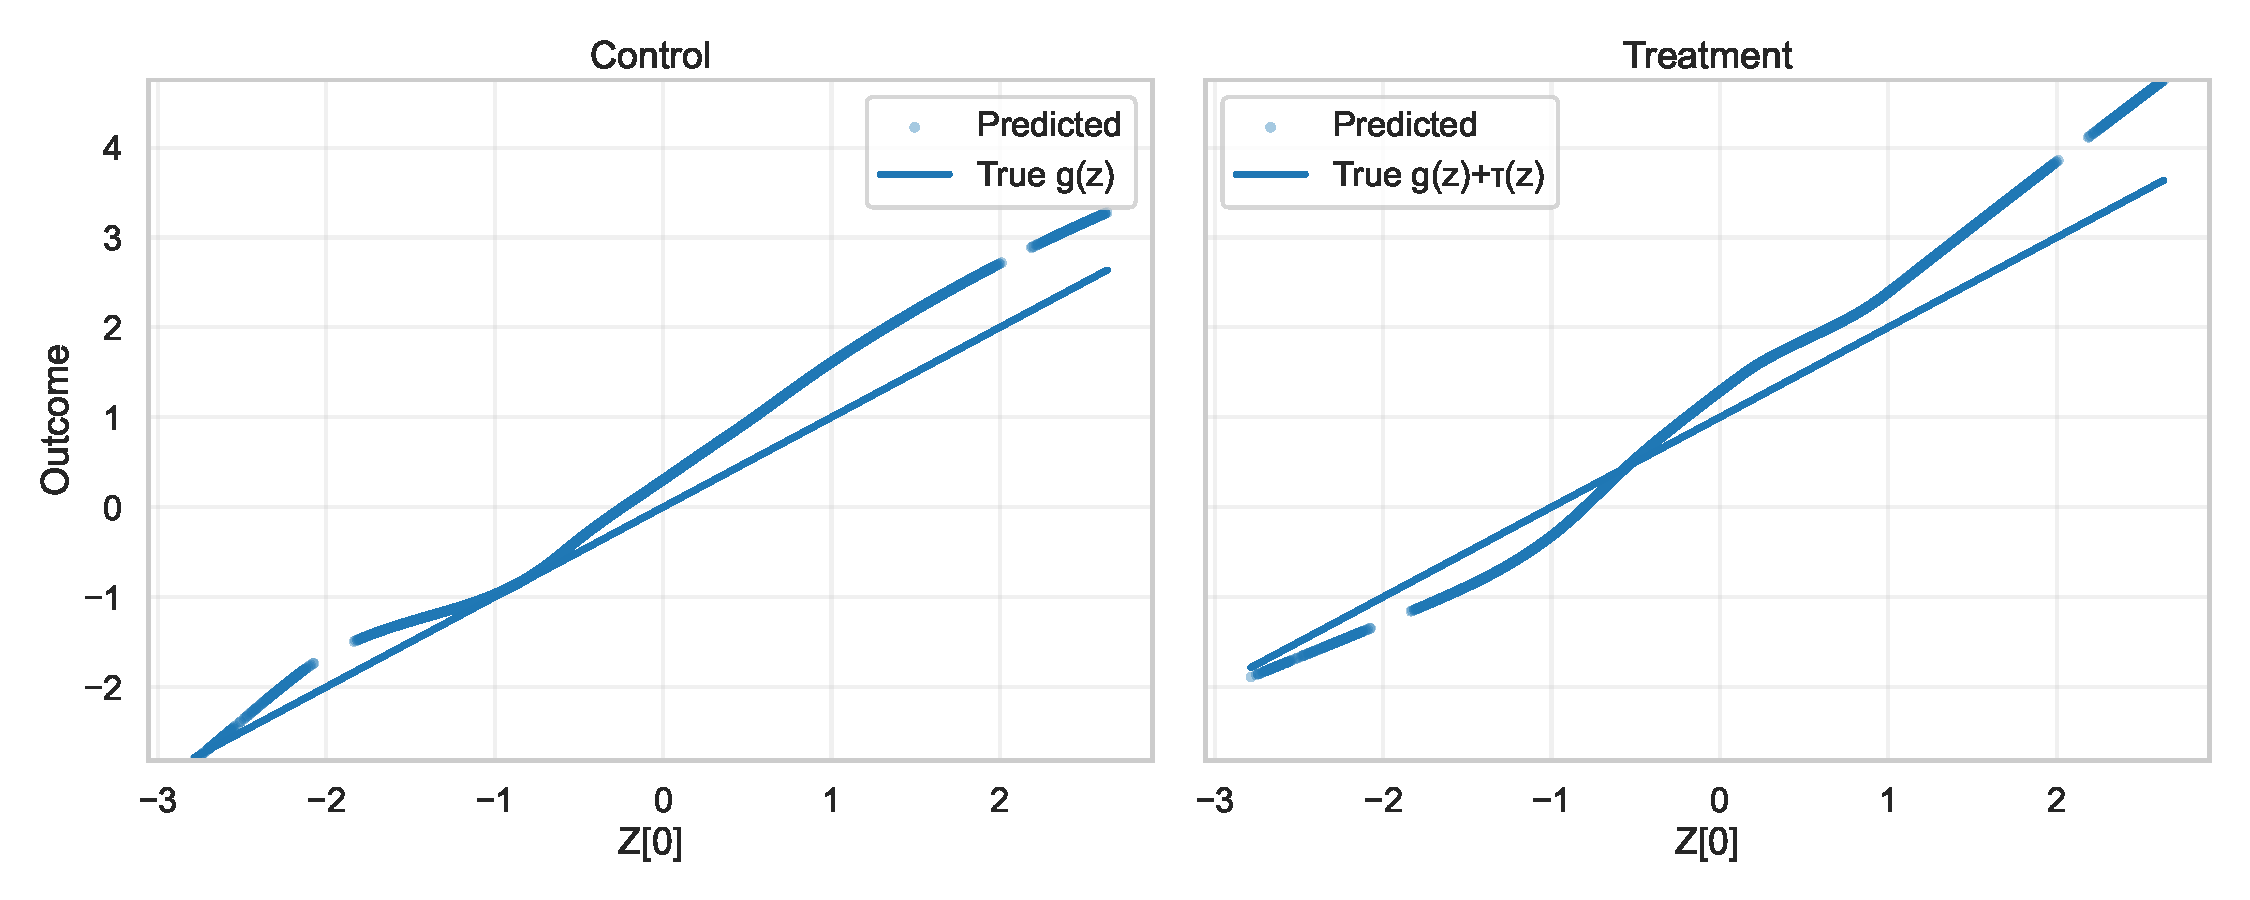
\includegraphics[width=\textwidth]{../src/results/linear_predicted_vs_true.pdf}
  \end{figure}  
\end{frame}

\begin{frame}{Internal Representation: Non Linear Dataset}
  \begin{figure}[H]
    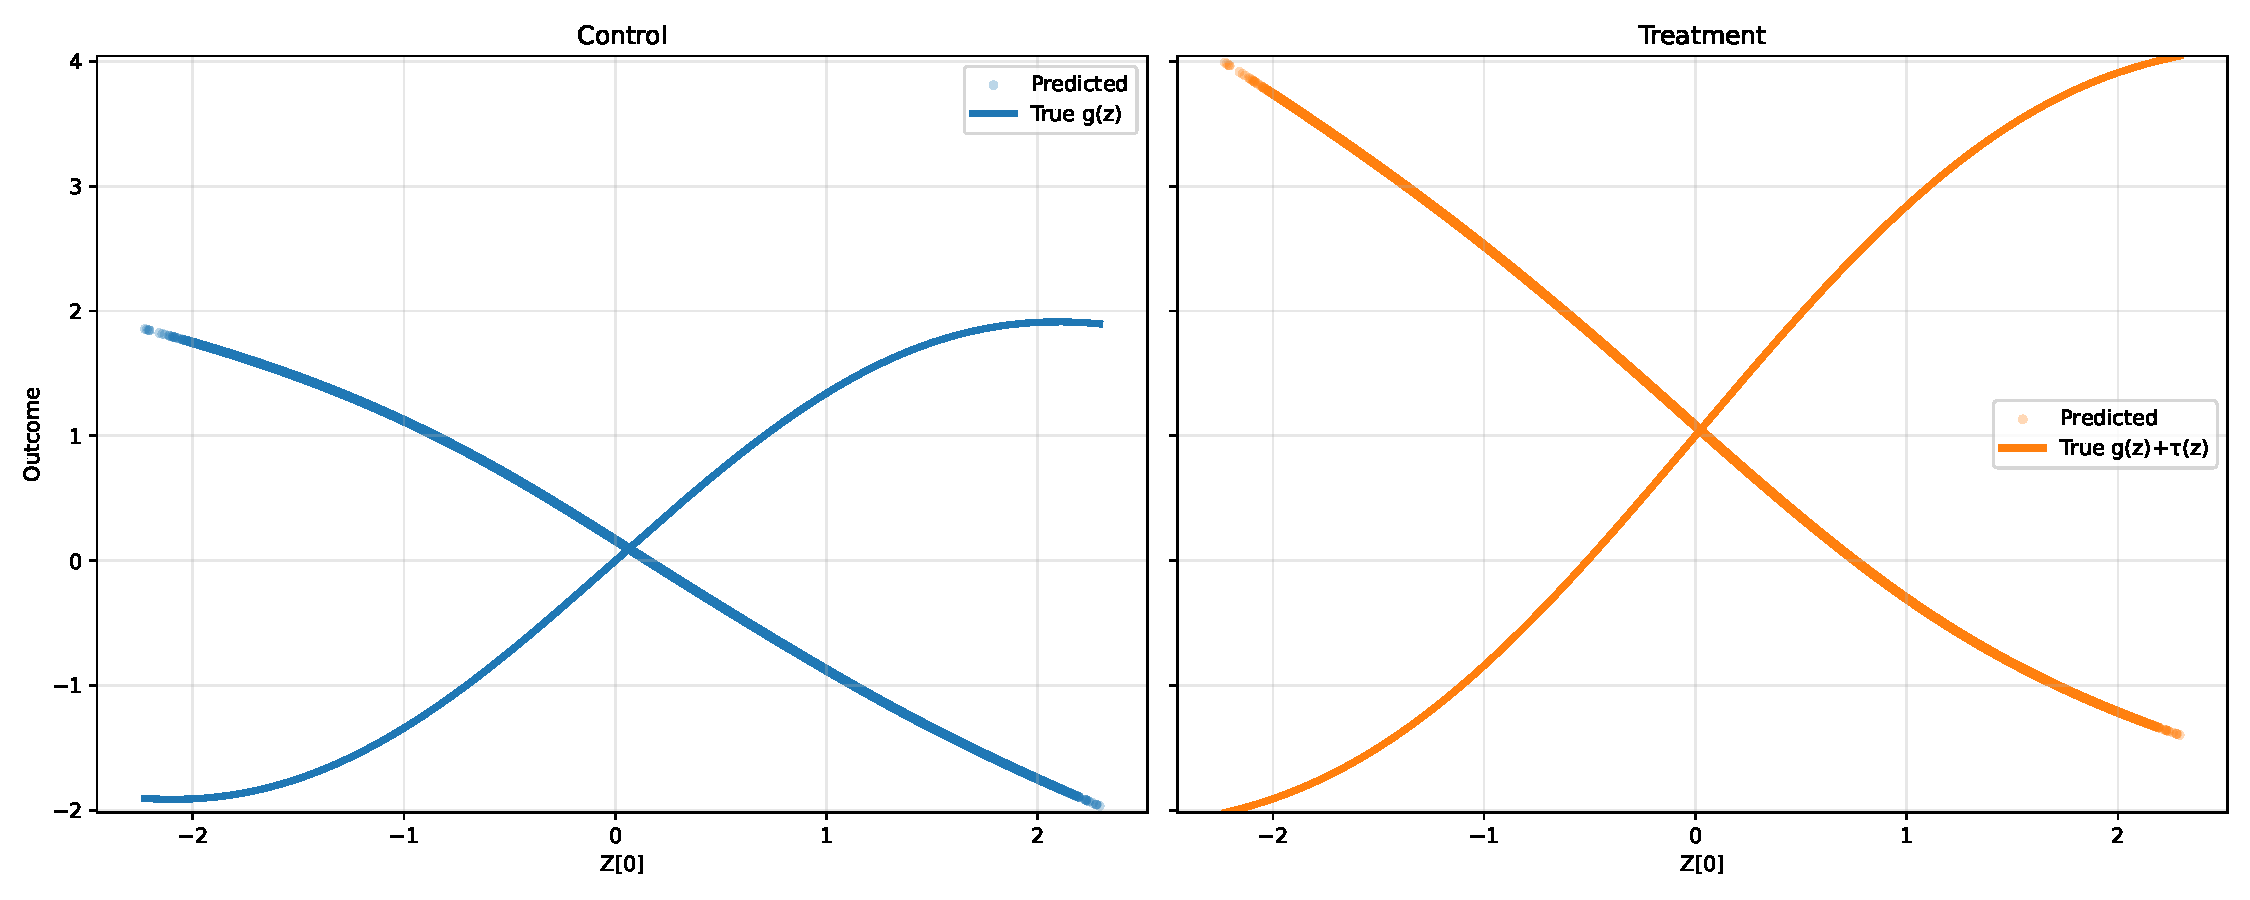
\includegraphics[width=\textwidth]{../src/results/non_linear_predicted_vs_true.pdf}
  \end{figure}  
\end{frame}

\begin{frame}{Experiment 1: Increasing the sample size}
  \begin{figure}[H]
      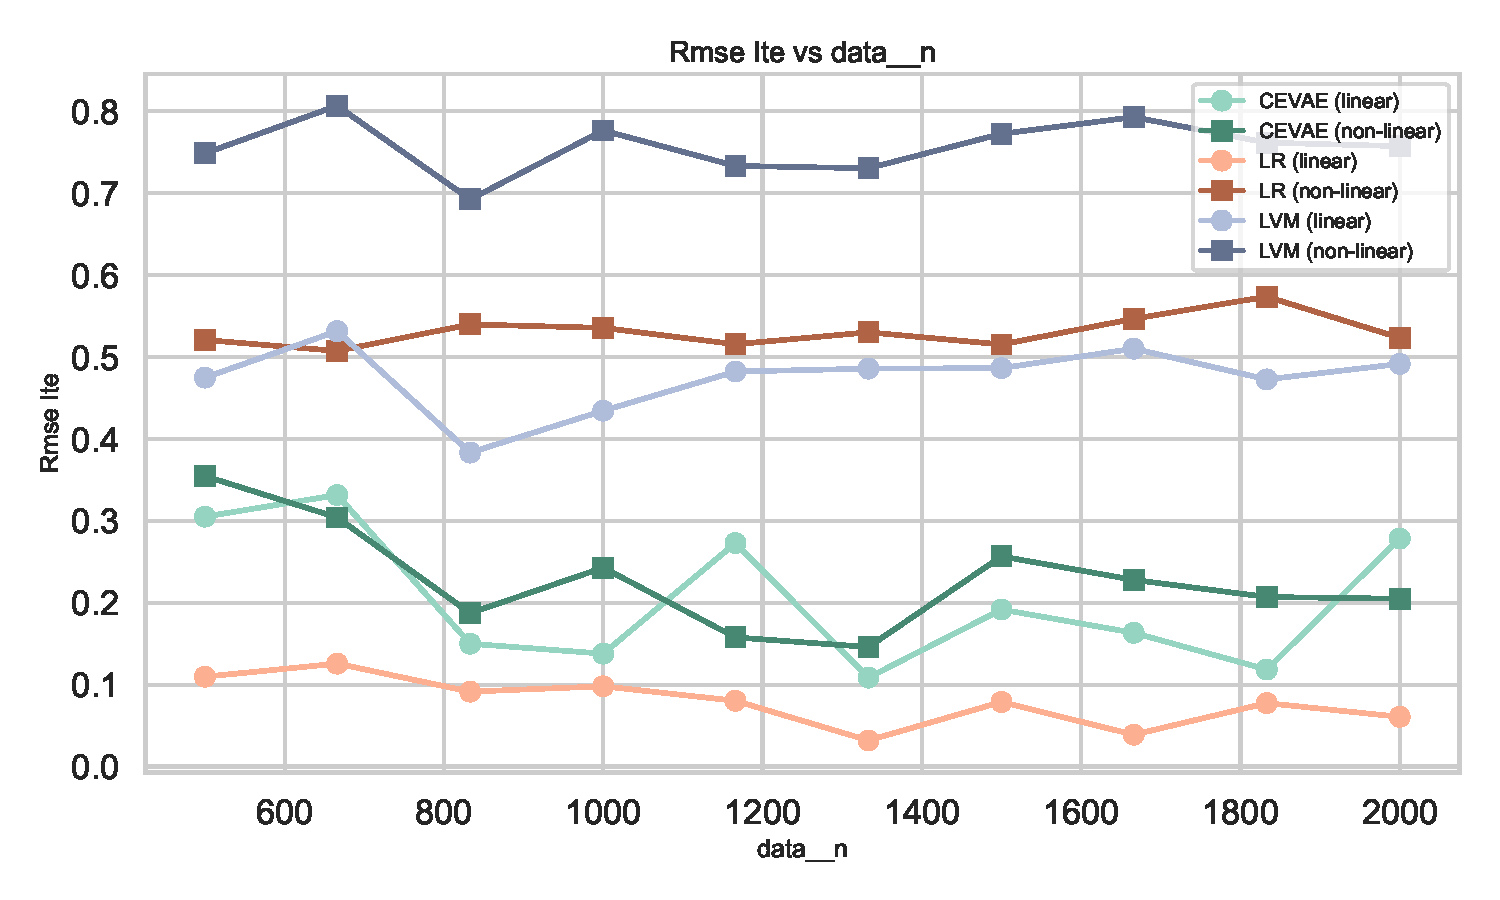
\includegraphics[width=\textwidth]{images/MyRun_data__n--rmse_ite.pdf}
    \end{figure}
\end{frame}

\begin{frame}{Experiment 2: Increasing decorrelation among proxies}
    \begin{figure}[H]
      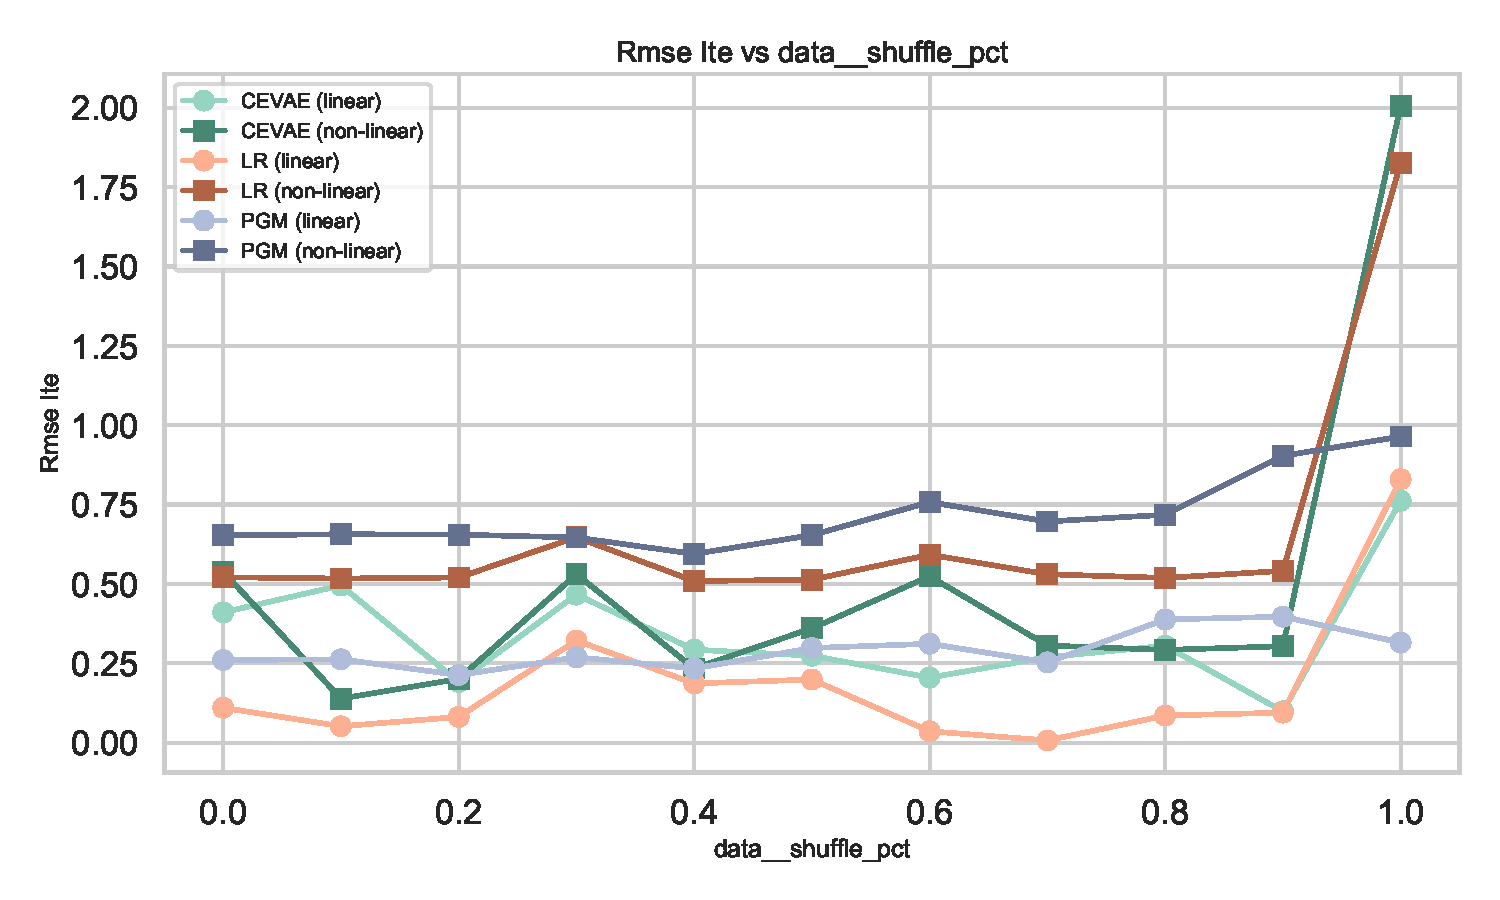
\includegraphics[width=\textwidth]{images/MyRun_data__shuffle_pct--rmse_ite.pdf}
    \end{figure}

\end{frame}

\begin{frame}{Experiment 3: Increasing latent dimension}
    \begin{figure}[H]
      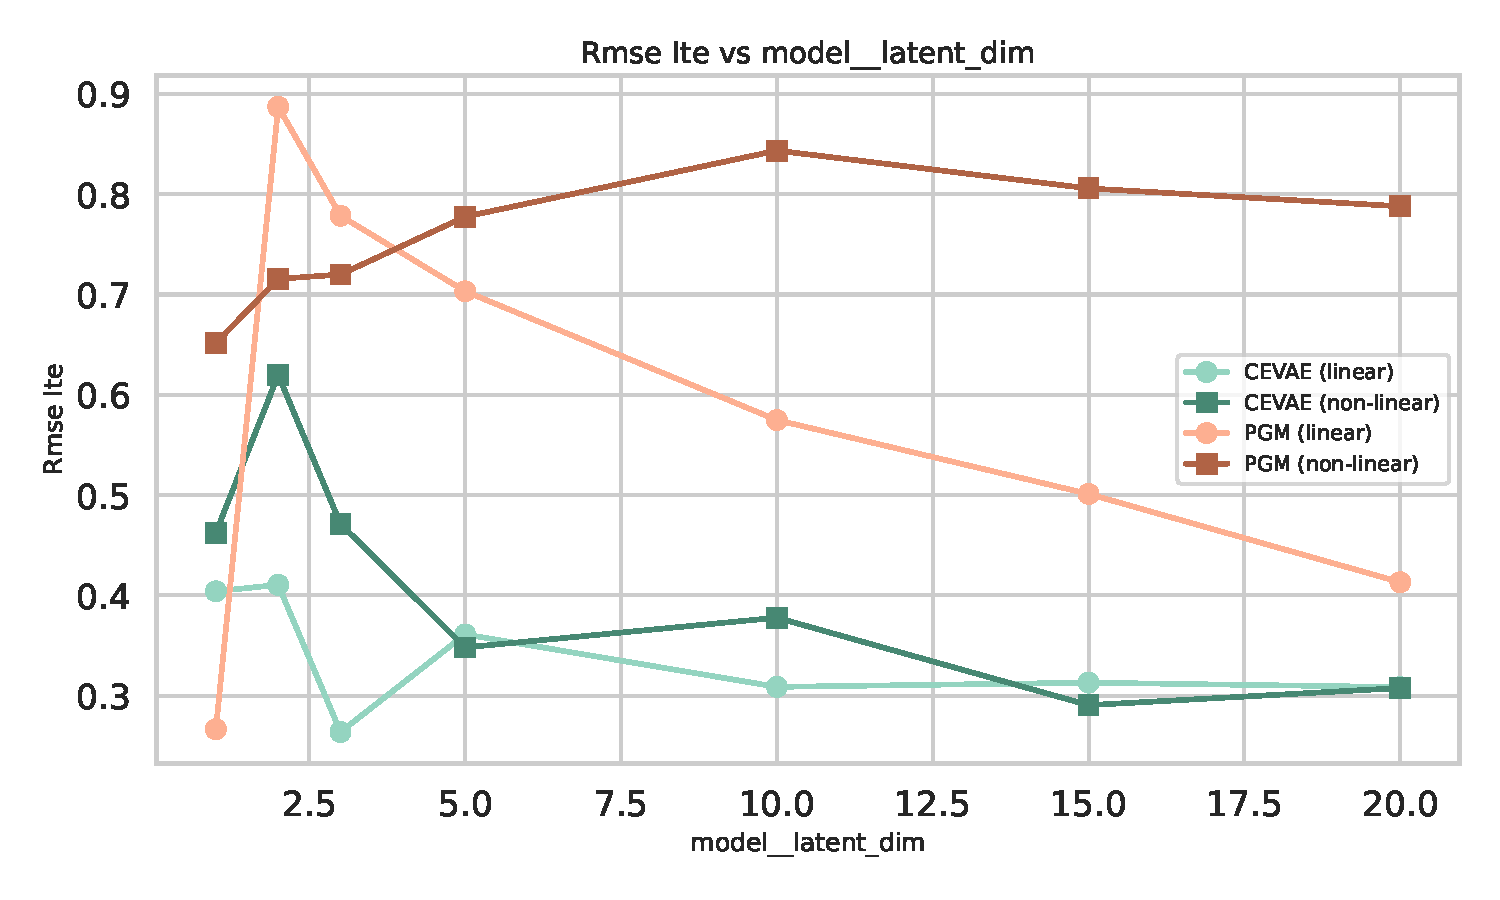
\includegraphics[width=\textwidth]{images/MyRun_model__latent_dim--rmse_ite.pdf}
    \end{figure}
\end{frame}

\begin{frame}{Experiment 4: latent distribution misspecified}
    \begin{figure}[H]
      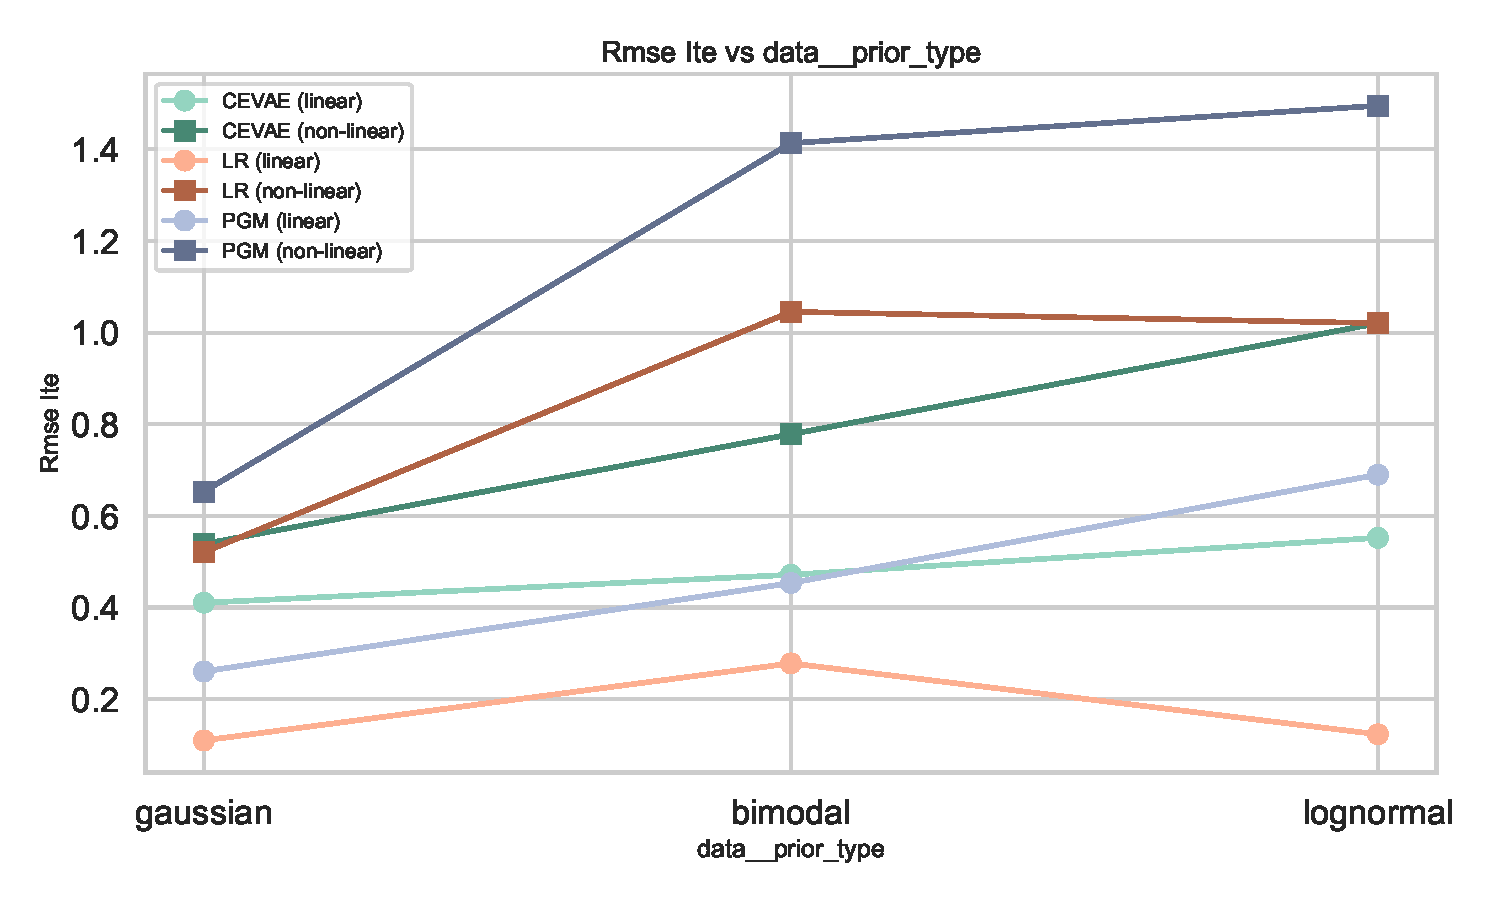
\includegraphics[width=\textwidth]{images/MyRun_data__prior_type--rmse_ite.pdf}
    \end{figure}
\end{frame}

\begin{frame}{Experiment 5: Increasing the number of proxies}
    \begin{figure}[H]
      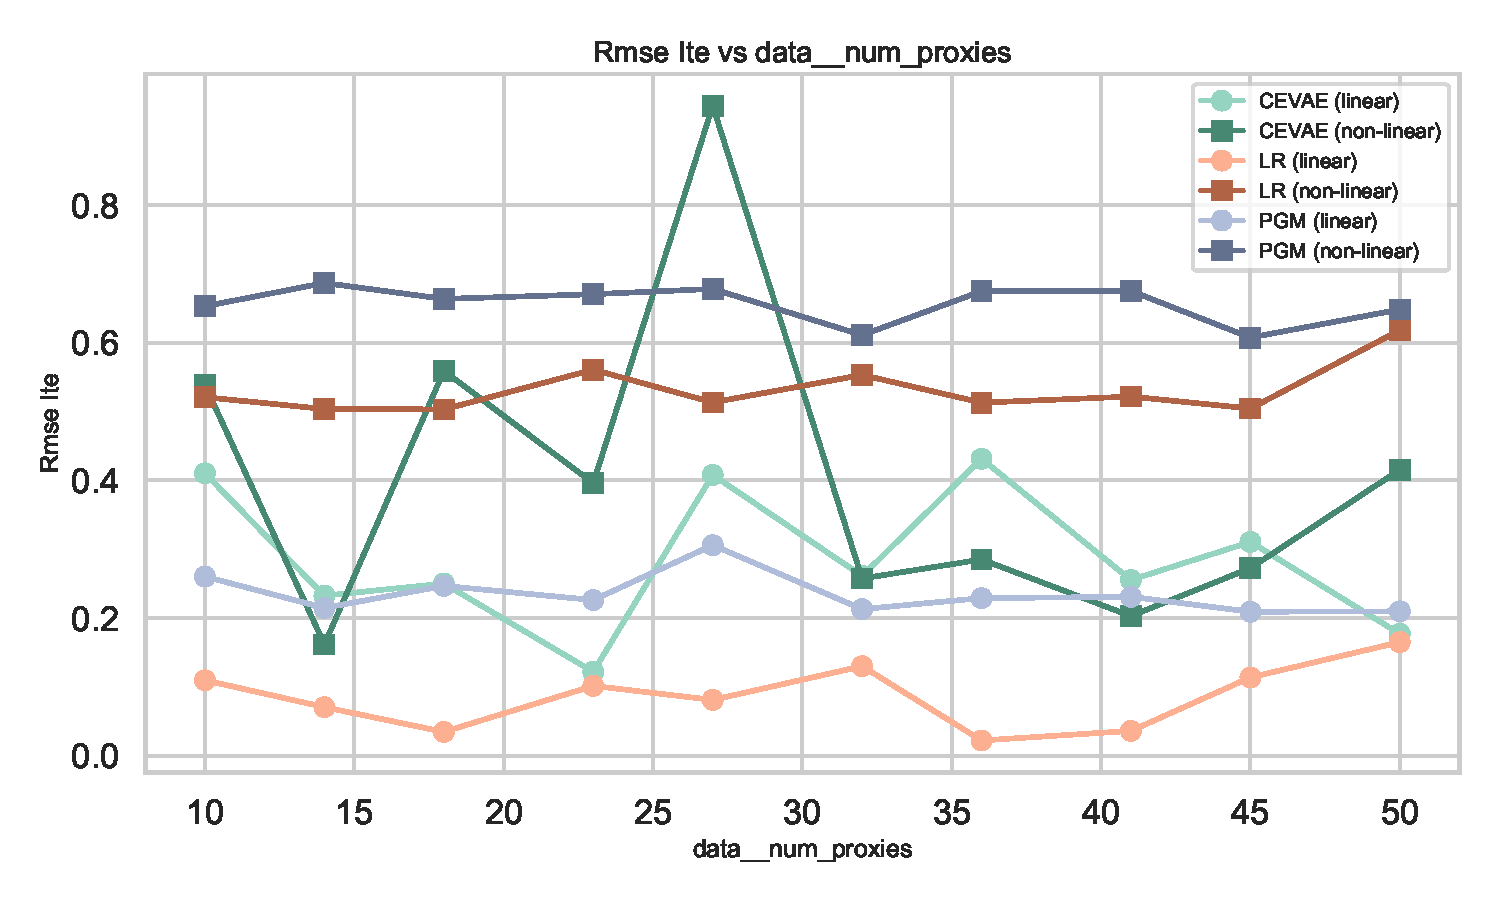
\includegraphics[width=\textwidth]{images/MyRun_data__num_proxies--rmse_ite.pdf}
    \end{figure}
\end{frame}

\begin{frame}{Conclusions}

\begin{itemize}\setlength\itemsep{6pt}

  \item \textbf{Linear synthetic data} -- 
        Linear models \emph{benefit} from strong prior assumptions and recover the true effects almost perfectly; CEVAE offers no gain and adds variance.

  \item \textbf{Non-linear synthetic data} -- 
        With a tuned latent dimension, CEVAE outperforms linear baselines; if untuned it over-fits and the latent loses causal meaning.

  \item \textbf{Practical takeaway}  
         -- Use simple models when you can state strong causal assumptions; switch to CEVAE to relax those assumptions—provided you can afford heavier training and tuning.

  \item \textbf{Next steps} -- 
        Test on real datasets, explore more sophisticate variant of CEVAE (e.g. \emph{TEDVAE}, \emph{DCEVAE}, \emph{ICEVAE})

\end{itemize}

\end{frame}

{\setbeamercolor{palette primary}{fg=white, bg=bluscuro}
\begin{frame}[standout]
\thispagestyle{empty}
  {\LARGE Thank You!}
\end{frame}
}

\end{document}